\documentclass[conference]{IEEEtran}

% ---- Packages ----
\usepackage{cite}
\usepackage{amsmath,amssymb,amsfonts}
\usepackage{graphicx}
\usepackage{textcomp}
\usepackage{xcolor}
\usepackage{booktabs}
\usepackage{multirow}
\usepackage{url}
\usepackage{hyperref}
\hypersetup{colorlinks=true, linkcolor=blue, citecolor=blue, urlcolor=blue}
\usepackage{tikz}
\usetikzlibrary{arrows.meta,positioning,fit,backgrounds,shapes.geometric}

% ---- TODO helper (remove before submission) ----
\newcommand{\TODO}[1]{\textcolor{red}{\textbf{[TODO: #1]}}}

\begin{document}

% -------------------------------------------------------
%  Title and Authors
% -------------------------------------------------------
\title{Efficient Road Damage Detection via RT-DETRv2:\\
Transformer-Based Detection with 70\% Fewer Parameters}

\author{
  \IEEEauthorblockN{Akarsh Hankumar}
  \IEEEauthorblockA{
    \textit{Department of \TODO{your department}}\\
    \TODO{Institution Name, City, Country}\\
    akarshhankumar003@gmail.com
  }
  % Add co-authors here if any
}

\maketitle

% -------------------------------------------------------
%  Abstract
% -------------------------------------------------------
\begin{abstract}
Road damage detection is a safety-critical infrastructure task that is costly and
inconsistent when performed manually at scale.
Convolutional neural network-based detectors such as RDD-YOLO achieve competitive
accuracy on the RDD2022 benchmark but carry prohibitive model sizes (65.9\,M
parameters, 255.3\,GFLOPs) that limit their use in resource-constrained deployment
scenarios.
We present a fine-tuned RT-DETRv2 model with a PResNet18 backbone trained on the
RDD2022 road damage dataset under a single-class formulation in which all four damage
categories (D00 longitudinal crack, D10 transverse crack, D20 alligator crack, D40
pothole) are treated as a unified \textit{road\_damage} class.
This formulation constitutes a harder generalisation benchmark than the per-class
setup used by prior work, as the detector must respond to all damage morphologies
without category-specific supervision.
Trained at 480$\times$480 resolution on the full RDD2022 dataset (17\,902 training
images), our model achieves mAP50\,=\,61.7\% and AR@50\,=\,92.6\% in 55 epochs,
compared to RDD-YOLO's mAP50\,=\,62.5\% trained for 180 epochs.
Critically, our model requires only approximately 20\,M parameters and 60\,GFLOPs,
representing a 70\% reduction in parameters and a 77\% reduction in compute relative
to RDD-YOLO.
An intermediate single-class model trained on a curated RDD2022 subset (5\,247 images)
achieves mAP50\,=\,80.3\%.
We further analyse model behaviour through Eigen-CAM activation maps and Deformable
Attention sampling-point visualisations, confirming that the backbone learns structural
damage features rather than road texture.
Our results demonstrate that transformer-based detection can match CNN-based accuracy
with substantially reduced computational cost on road damage benchmarks.
\end{abstract}

\begin{IEEEkeywords}
road damage detection, transformer detection, RT-DETRv2, RDD2022, deformable attention,
single-class detection, efficient object detection
\end{IEEEkeywords}

% -------------------------------------------------------
%  1. Introduction
% -------------------------------------------------------
\section{Introduction}

Road infrastructure deterioration is a global challenge with significant safety and
economic consequences.
According to the World Health Organization, poor road conditions are a contributing
factor in a substantial share of traffic fatalities worldwide~\cite{who2023roads}.
Manual inspection of road networks is labour-intensive, geographically inconsistent,
and increasingly impractical as infrastructure inventories grow.
Camera-based automated detection using deep learning has emerged as a scalable
alternative for continuous road condition monitoring.

Existing deep learning detectors applied to the RDD2022 benchmark~\cite{arya2022rdd}
have focused predominantly on YOLO-series convolutional architectures.
The state-of-the-art CNN baseline RDD-YOLO~\cite{rddyolo} employs a YOLOv8x backbone
augmented with SimAM attention~\cite{yang2021simam} and GhostConv~\cite{han2020ghost}
neck modifications, achieving mAP50\,=\,62.5\% at the cost of 65.9\,M parameters and
255.3\,GFLOPs per inference pass.
Transformer-based detectors, which have achieved strong results on general-purpose
benchmarks, remain underexplored on the RDD2022 road damage benchmark.

This paper investigates RT-DETRv2~\cite{chen2024rtdetrv2}, a real-time end-to-end
transformer detector, fine-tuned on RDD2022.
We adopt a single-class formulation that collapses all four damage type annotations
into a single \textit{road\_damage} category.
This is a deliberately harder benchmark than per-class evaluation: without category
cues, the model must detect longitudinal cracks, transverse cracks, alligator cracks,
and potholes through structural feature extraction alone.

The contributions of this paper are:
\begin{enumerate}
  \item The first application of RT-DETRv2 to the RDD2022 road damage benchmark.
  \item A single-class collapse strategy that generalises across all damage
        morphologies in the dataset.
  \item An efficiency analysis demonstrating 70\% fewer parameters and 77\% fewer
        GFLOPs than RDD-YOLO at near-equivalent mAP50.
  \item Interpretability analysis via Eigen-CAM and Deformable Attention
        visualisation confirming structural feature learning.
\end{enumerate}

The remainder of this paper is organised as follows.
Section~\ref{sec:related} reviews related work.
Section~\ref{sec:dataset} describes the dataset and problem formulation.
Section~\ref{sec:method} presents the methodology.
Section~\ref{sec:experiments} reports experiments and results.
Section~\ref{sec:discussion} discusses findings and limitations.
Section~\ref{sec:conclusion} concludes.

% -------------------------------------------------------
%  2. Related Work
% -------------------------------------------------------
\section{Related Work}
\label{sec:related}

\subsection{CNN-Based Road Damage Detection}

Automated road damage detection has been studied extensively since the release of the
RDD2018 and RDD2020 datasets~\cite{maeda2018rdd}.
YOLO-series detectors have been widely adopted for this task due to their
single-stage speed characteristics.
RDD-YOLO~\cite{rddyolo} represents the current CNN state of the art on RDD2022,
combining a YOLOv8x backbone~\cite{jocher2023yolov8} with SimAM channel
attention~\cite{yang2021simam}, a GhostConv~\cite{han2020ghost} feature pyramid neck,
and bilinear upsampling.
Trained on RDD2022 for 180 epochs at 640$\times$640 resolution, it achieves
mAP50\,=\,62.5\% across four damage classes.
However, its 65.9\,M parameter count and 255.3\,GFLOPs present barriers to
deployment on platforms with constrained compute budgets.
Lightweight CNN alternatives have been explored for embedded road inspection,
including MobiLiteNet~\cite{hu2025lightweight}, but typically exhibit a larger
accuracy penalty than the approach we present here.

\subsection{Transformer-Based Object Detection}

DETR~\cite{carion2020detr} introduced end-to-end object detection via a transformer
encoder--decoder architecture, eliminating the need for hand-crafted anchor generation
and non-maximum suppression.
Deformable DETR~\cite{zhu2021deformable} extended this with deformable attention,
attending to a small set of learned sampling points rather than all spatial positions,
substantially reducing convergence time.
RT-DETR~\cite{lyu2023rtdetr} and its successor RT-DETRv2~\cite{chen2024rtdetrv2}
further improve real-time performance through a hybrid CNN--transformer encoder
combining a convolutional backbone with an Asymptotic Feature Interaction (AIFI)
module for multi-scale feature fusion.
RT-DETRv2 additionally introduces IoU-aware query selection and decoupled contrastive
denoising training, improving detection quality without increasing inference cost.
To our knowledge, no prior work has evaluated RT-DETRv2 on the RDD2022 benchmark.

\subsection{Transfer Learning for Detection}

Transfer learning from large datasets such as COCO~\cite{lin2014coco} is standard
practice for domain-specific detection.
Full fine-tuning of all backbone and decoder parameters consistently outperforms
partial-freeze approaches when the target domain differs substantially from the
pre-training domain~\cite{zaidi2022survey}---a finding confirmed in our own
preliminary experiments.
Multi-scale training, in which different input resolutions are sampled during training,
has been shown to improve detection of small objects~\cite{lin2017fpn}.

\subsection{Explainability in Detection Models}

Grad-CAM~\cite{selvaraju2017gradcam} and its gradient-free variant
Eigen-CAM~\cite{muhammad2020eigencam} have been widely used to visualise which spatial
regions drive convolutional feature activations.
For transformer-based detectors, visualisation of deformable attention sampling
points~\cite{zhu2021deformable} provides a complementary view of where the decoder
attends when predicting bounding boxes.
Explainability work specifically targeted at road damage detection models is
limited~\cite{guo2025xai}, making our analysis a useful contribution for
understanding model behaviour in safety-critical inspection contexts.

% -------------------------------------------------------
%  3. Dataset and Problem Formulation
% -------------------------------------------------------
\section{Dataset and Problem Formulation}
\label{sec:dataset}

\subsection{RDD2022 Dataset}

The Road Damage Dataset 2022 (RDD2022)~\cite{arya2022rdd} is a large-scale
multi-country road damage benchmark comprising images collected across Japan, India,
the Czech Republic, Norway, the United States, and China under diverse weather and
road surface conditions.
Annotations cover four damage categories:
\textbf{D00} (longitudinal cracks),
\textbf{D10} (transverse cracks),
\textbf{D20} (alligator/mesh cracks), and
\textbf{D40} (potholes).
We use the cleaned training split sourced from RDD2022 (17\,902 training images with
valid bounding boxes; 3\,743 validation images).

\subsection{Single-Class Reformulation}

Rather than training a separate output head for each damage category, we collapse all
four annotation types to a single \textit{road\_damage} class.
This formulation serves two purposes.
First, it reflects the primary operational requirement of many road inspection
systems: detecting the \emph{presence} of damage, rather than its precise type, to
trigger further assessment.
Second, inter-annotator boundary ambiguity between closely related categories (e.g.\
D00 and D10 in aged or multi-directional cracking) introduces label noise that the
single-class formulation avoids.

We acknowledge the principal trade-off: the single-class detector cannot provide
per-category severity reports useful for infrastructure management databases.
However, our evaluation demonstrates that this formulation achieves strong detection
recall across all damage morphologies without category-specific supervision, making it
appropriate for detection and alerting applications.

\subsection{Evaluation Metrics}

We report metrics following the COCO evaluation protocol~\cite{lin2014coco}:
\begin{itemize}
  \item \textbf{mAP50} -- mean Average Precision at IoU threshold 0.50.
  \item \textbf{mAP50-95} -- mean AP averaged over IoU thresholds 0.50--0.95 in
        steps of 0.05.
  \item \textbf{AR@50} -- Average Recall at IoU threshold 0.50, averaged over
        detections per image.
  \item \textbf{AP$_\text{small}$} -- AP for objects with area $<32^2$ pixels.
\end{itemize}

We treat AR@50 as our primary safety-critical metric.
In a road inspection context, a missed detection (false negative) carries a higher
operational cost than a spurious detection (false positive), since undetected damage
may go unrepaired and pose a hazard.
An AR@50 of 0.926 means fewer than 8\% of damage instances are missed at an IoU
threshold of 0.50.

% -------------------------------------------------------
%  4. Methodology
% -------------------------------------------------------
\section{Methodology}
\label{sec:method}

\subsection{RT-DETRv2 Architecture}

RT-DETRv2~\cite{chen2024rtdetrv2} is an end-to-end real-time object detector that
combines a convolutional backbone with a transformer encoder--decoder, eliminating the
need for non-maximum suppression at inference.

\textbf{Backbone.}
We use PResNet18, a parameterised-residual variant of ResNet-18, as the feature
extractor.
PResNet18 contains approximately 20\,M parameters in total when combined with the
encoder and decoder, compared to 65.9\,M for the YOLOv8x backbone used in
RDD-YOLO~\cite{rddyolo}.
Multi-scale feature maps at three scales (stride 8, 16, 32) are extracted from the
backbone and passed to the encoder.

\textbf{Encoder.}
The Asymptotic Feature Interaction (AIFI) module performs intra-scale self-attention
at the highest-level feature map before a channel-projection cross-scale fusion step
produces the multi-scale encoder output.
This hybrid design avoids the quadratic cost of full cross-scale transformer
attention.

\textbf{Decoder.}
The transformer decoder comprises 3 layers (reduced from the default 6 for
efficiency) with deformable cross-attention~\cite{zhu2021deformable} operating in
discrete mode, which produces sampling offsets discretised to grid positions and is
compatible with efficient inference pipelines.
We use 100 object queries.
IoU-aware query selection~\cite{chen2024rtdetrv2} initialises queries from the
encoder output regions with highest foreground confidence, accelerating convergence.
Decoupled contrastive denoising is applied during training to stabilise the
bipartite matching.

An architectural overview is shown in Fig.~\ref{fig:architecture}.

\begin{figure}[t]
  \centering
  \resizebox{\columnwidth}{!}{% architecture.tex — RT-DETRv2 architecture diagram for inclusion in main.tex
% Include with: % architecture.tex — RT-DETRv2 architecture diagram for inclusion in main.tex
% Include with: % architecture.tex — RT-DETRv2 architecture diagram for inclusion in main.tex
% Include with: \input{figures/architecture}
%
% Required packages in main.tex preamble:
%   \usepackage{tikz}
%   \usetikzlibrary{arrows.meta, positioning, fit, backgrounds, shapes.geometric}

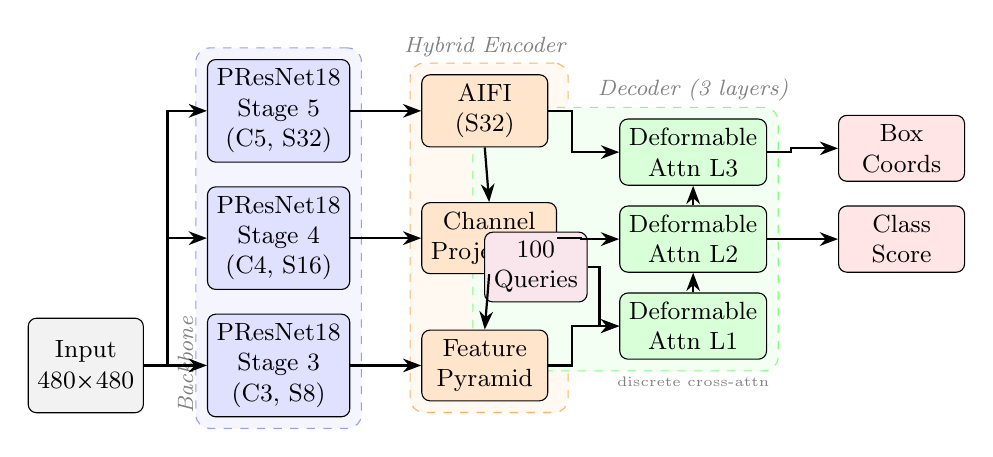
\begin{tikzpicture}[
  font=\small,
  >=Stealth,
  % Block styles
  backbone/.style={
    draw, fill=blue!12, rounded corners=3pt,
    minimum width=1.6cm, minimum height=0.65cm, align=center
  },
  encoder/.style={
    draw, fill=orange!20, rounded corners=3pt,
    minimum width=1.6cm, minimum height=0.65cm, align=center
  },
  decoder/.style={
    draw, fill=green!15, rounded corners=3pt,
    minimum width=1.6cm, minimum height=0.65cm, align=center
  },
  output/.style={
    draw, fill=red!10, rounded corners=3pt,
    minimum width=1.6cm, minimum height=0.65cm, align=center
  },
  arrow/.style={->, thick},
  label/.style={font=\footnotesize\itshape, text=gray}
]

% ── Input image ──────────────────────────────────────────────────────────────
\node[draw, fill=gray!10, rounded corners=3pt,
      minimum width=1.2cm, minimum height=1.2cm, align=center] (img)
      {Input\\480\texttimes480};

% ── Backbone: PResNet18 ───────────────────────────────────────────────────────
\node[backbone, right=0.8cm of img] (bb1) {PResNet18\\Stage 3\\(C3, S8)};
\node[backbone, above=0.3cm of bb1] (bb2) {PResNet18\\Stage 4\\(C4, S16)};
\node[backbone, above=0.3cm of bb2] (bb3) {PResNet18\\Stage 5\\(C5, S32)};

% Backbone group label
\node[label, left=0.05cm of bb1, rotate=90, anchor=south] {Backbone};

% ── Encoder: AIFI + projection ───────────────────────────────────────────────
\node[encoder, right=0.9cm of bb3] (aifi) {AIFI\\(S32)};
\node[encoder, right=0.9cm of bb2] (proj) {Channel\\Projection};
\node[encoder, right=0.9cm of bb1] (fpn)  {Feature\\Pyramid};

% Encoder group label
\node[label, above=0.1cm of aifi] {Hybrid Encoder};

% ── Decoder ──────────────────────────────────────────────────────────────────
\node[decoder, right=0.9cm of fpn, yshift=0.5cm] (dec1) {Deformable\\Attn L1};
\node[decoder, above=0.25cm of dec1]              (dec2) {Deformable\\Attn L2};
\node[decoder, above=0.25cm of dec2]              (dec3) {Deformable\\Attn L3};

% Decoder group label
\node[label, above=0.1cm of dec3] {Decoder (3 layers)};

% Queries box
\node[draw, fill=purple!10, rounded corners=3pt,
      minimum width=1.2cm, minimum height=0.5cm, align=center,
      left=0.4cm of dec1, yshift=0.75cm] (q) {100\\Queries};

% ── Output heads ─────────────────────────────────────────────────────────────
\node[output, right=0.9cm of dec2] (cls) {Class\\Score};
\node[output, above=0.3cm of cls]  (box) {Box\\Coords};

% ── Arrows: image -> backbone ─────────────────────────────────────────────────
\draw[arrow] (img.east) -- ++(0.3,0) |- (bb1.west);
\draw[arrow] (img.east) -- ++(0.3,0) |- (bb2.west);
\draw[arrow] (img.east) -- ++(0.3,0) |- (bb3.west);

% ── Arrows: backbone -> encoder ───────────────────────────────────────────────
\draw[arrow] (bb3.east) -- (aifi.west);
\draw[arrow] (bb2.east) -- (proj.west);
\draw[arrow] (bb1.east) -- (fpn.west);
\draw[arrow] (aifi.south) -- (proj.north);
\draw[arrow] (proj.south) -- (fpn.north);

% ── Arrows: encoder -> decoder ────────────────────────────────────────────────
\draw[arrow] (fpn.east)  -- ++(0.3,0) |- (dec1.west);
\draw[arrow] (proj.east) -- ++(0.3,0) |- (dec2.west);
\draw[arrow] (aifi.east) -- ++(0.3,0) |- (dec3.west);

% ── Queries -> decoder ────────────────────────────────────────────────────────
\draw[arrow] (q.east) -- ++(0.15,0) |- (dec1.west);

% ── Decoder chain ─────────────────────────────────────────────────────────────
\draw[arrow] (dec1.north) -- (dec2.south);
\draw[arrow] (dec2.north) -- (dec3.south);

% ── Decoder -> output ─────────────────────────────────────────────────────────
\draw[arrow] (dec3.east) -- ++(0.3,0) |- (box.west);
\draw[arrow] (dec2.east) -- ++(0.3,0) |- (cls.west);

% ── Background boxes (visual grouping) ───────────────────────────────────────
\begin{scope}[on background layer]
  \node[draw=blue!40, dashed, fill=blue!4, rounded corners=5pt,
        fit=(bb1)(bb2)(bb3), inner sep=4pt] {};
  \node[draw=orange!60, dashed, fill=orange!5, rounded corners=5pt,
        fit=(aifi)(proj)(fpn), inner sep=4pt] {};
  \node[draw=green!50, dashed, fill=green!5, rounded corners=5pt,
        fit=(dec1)(dec2)(dec3)(q), inner sep=4pt] {};
\end{scope}

% ── Annotation: discrete cross-attention ─────────────────────────────────────
\node[font=\tiny, text=gray, align=center, below=0.1cm of dec1]
  {discrete cross-attn};

\end{tikzpicture}

%
% Required packages in main.tex preamble:
%   \usepackage{tikz}
%   \usetikzlibrary{arrows.meta, positioning, fit, backgrounds, shapes.geometric}

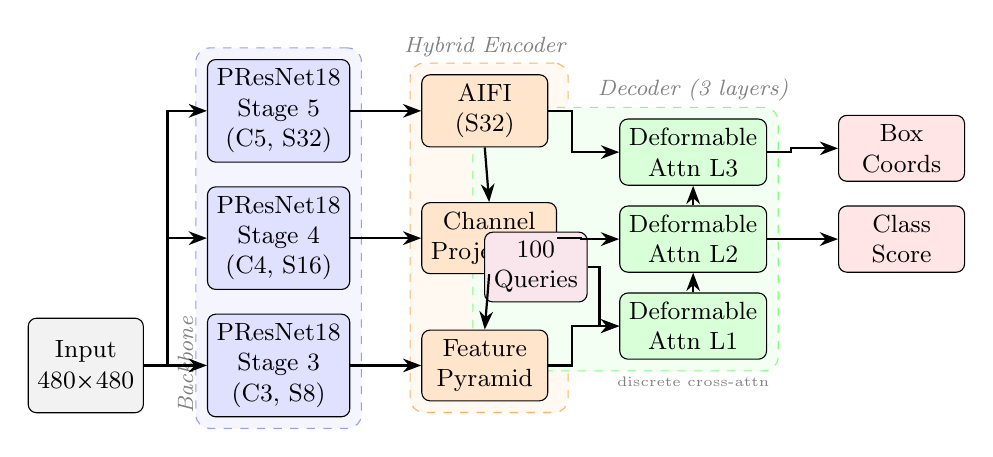
\begin{tikzpicture}[
  font=\small,
  >=Stealth,
  % Block styles
  backbone/.style={
    draw, fill=blue!12, rounded corners=3pt,
    minimum width=1.6cm, minimum height=0.65cm, align=center
  },
  encoder/.style={
    draw, fill=orange!20, rounded corners=3pt,
    minimum width=1.6cm, minimum height=0.65cm, align=center
  },
  decoder/.style={
    draw, fill=green!15, rounded corners=3pt,
    minimum width=1.6cm, minimum height=0.65cm, align=center
  },
  output/.style={
    draw, fill=red!10, rounded corners=3pt,
    minimum width=1.6cm, minimum height=0.65cm, align=center
  },
  arrow/.style={->, thick},
  label/.style={font=\footnotesize\itshape, text=gray}
]

% ── Input image ──────────────────────────────────────────────────────────────
\node[draw, fill=gray!10, rounded corners=3pt,
      minimum width=1.2cm, minimum height=1.2cm, align=center] (img)
      {Input\\480\texttimes480};

% ── Backbone: PResNet18 ───────────────────────────────────────────────────────
\node[backbone, right=0.8cm of img] (bb1) {PResNet18\\Stage 3\\(C3, S8)};
\node[backbone, above=0.3cm of bb1] (bb2) {PResNet18\\Stage 4\\(C4, S16)};
\node[backbone, above=0.3cm of bb2] (bb3) {PResNet18\\Stage 5\\(C5, S32)};

% Backbone group label
\node[label, left=0.05cm of bb1, rotate=90, anchor=south] {Backbone};

% ── Encoder: AIFI + projection ───────────────────────────────────────────────
\node[encoder, right=0.9cm of bb3] (aifi) {AIFI\\(S32)};
\node[encoder, right=0.9cm of bb2] (proj) {Channel\\Projection};
\node[encoder, right=0.9cm of bb1] (fpn)  {Feature\\Pyramid};

% Encoder group label
\node[label, above=0.1cm of aifi] {Hybrid Encoder};

% ── Decoder ──────────────────────────────────────────────────────────────────
\node[decoder, right=0.9cm of fpn, yshift=0.5cm] (dec1) {Deformable\\Attn L1};
\node[decoder, above=0.25cm of dec1]              (dec2) {Deformable\\Attn L2};
\node[decoder, above=0.25cm of dec2]              (dec3) {Deformable\\Attn L3};

% Decoder group label
\node[label, above=0.1cm of dec3] {Decoder (3 layers)};

% Queries box
\node[draw, fill=purple!10, rounded corners=3pt,
      minimum width=1.2cm, minimum height=0.5cm, align=center,
      left=0.4cm of dec1, yshift=0.75cm] (q) {100\\Queries};

% ── Output heads ─────────────────────────────────────────────────────────────
\node[output, right=0.9cm of dec2] (cls) {Class\\Score};
\node[output, above=0.3cm of cls]  (box) {Box\\Coords};

% ── Arrows: image -> backbone ─────────────────────────────────────────────────
\draw[arrow] (img.east) -- ++(0.3,0) |- (bb1.west);
\draw[arrow] (img.east) -- ++(0.3,0) |- (bb2.west);
\draw[arrow] (img.east) -- ++(0.3,0) |- (bb3.west);

% ── Arrows: backbone -> encoder ───────────────────────────────────────────────
\draw[arrow] (bb3.east) -- (aifi.west);
\draw[arrow] (bb2.east) -- (proj.west);
\draw[arrow] (bb1.east) -- (fpn.west);
\draw[arrow] (aifi.south) -- (proj.north);
\draw[arrow] (proj.south) -- (fpn.north);

% ── Arrows: encoder -> decoder ────────────────────────────────────────────────
\draw[arrow] (fpn.east)  -- ++(0.3,0) |- (dec1.west);
\draw[arrow] (proj.east) -- ++(0.3,0) |- (dec2.west);
\draw[arrow] (aifi.east) -- ++(0.3,0) |- (dec3.west);

% ── Queries -> decoder ────────────────────────────────────────────────────────
\draw[arrow] (q.east) -- ++(0.15,0) |- (dec1.west);

% ── Decoder chain ─────────────────────────────────────────────────────────────
\draw[arrow] (dec1.north) -- (dec2.south);
\draw[arrow] (dec2.north) -- (dec3.south);

% ── Decoder -> output ─────────────────────────────────────────────────────────
\draw[arrow] (dec3.east) -- ++(0.3,0) |- (box.west);
\draw[arrow] (dec2.east) -- ++(0.3,0) |- (cls.west);

% ── Background boxes (visual grouping) ───────────────────────────────────────
\begin{scope}[on background layer]
  \node[draw=blue!40, dashed, fill=blue!4, rounded corners=5pt,
        fit=(bb1)(bb2)(bb3), inner sep=4pt] {};
  \node[draw=orange!60, dashed, fill=orange!5, rounded corners=5pt,
        fit=(aifi)(proj)(fpn), inner sep=4pt] {};
  \node[draw=green!50, dashed, fill=green!5, rounded corners=5pt,
        fit=(dec1)(dec2)(dec3)(q), inner sep=4pt] {};
\end{scope}

% ── Annotation: discrete cross-attention ─────────────────────────────────────
\node[font=\tiny, text=gray, align=center, below=0.1cm of dec1]
  {discrete cross-attn};

\end{tikzpicture}

%
% Required packages in main.tex preamble:
%   \usepackage{tikz}
%   \usetikzlibrary{arrows.meta, positioning, fit, backgrounds, shapes.geometric}

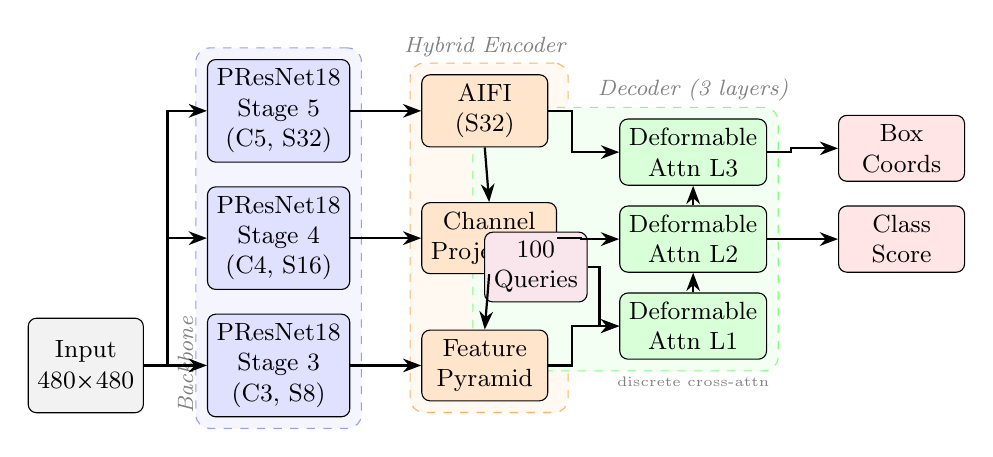
\begin{tikzpicture}[
  font=\small,
  >=Stealth,
  % Block styles
  backbone/.style={
    draw, fill=blue!12, rounded corners=3pt,
    minimum width=1.6cm, minimum height=0.65cm, align=center
  },
  encoder/.style={
    draw, fill=orange!20, rounded corners=3pt,
    minimum width=1.6cm, minimum height=0.65cm, align=center
  },
  decoder/.style={
    draw, fill=green!15, rounded corners=3pt,
    minimum width=1.6cm, minimum height=0.65cm, align=center
  },
  output/.style={
    draw, fill=red!10, rounded corners=3pt,
    minimum width=1.6cm, minimum height=0.65cm, align=center
  },
  arrow/.style={->, thick},
  label/.style={font=\footnotesize\itshape, text=gray}
]

% ── Input image ──────────────────────────────────────────────────────────────
\node[draw, fill=gray!10, rounded corners=3pt,
      minimum width=1.2cm, minimum height=1.2cm, align=center] (img)
      {Input\\480\texttimes480};

% ── Backbone: PResNet18 ───────────────────────────────────────────────────────
\node[backbone, right=0.8cm of img] (bb1) {PResNet18\\Stage 3\\(C3, S8)};
\node[backbone, above=0.3cm of bb1] (bb2) {PResNet18\\Stage 4\\(C4, S16)};
\node[backbone, above=0.3cm of bb2] (bb3) {PResNet18\\Stage 5\\(C5, S32)};

% Backbone group label
\node[label, left=0.05cm of bb1, rotate=90, anchor=south] {Backbone};

% ── Encoder: AIFI + projection ───────────────────────────────────────────────
\node[encoder, right=0.9cm of bb3] (aifi) {AIFI\\(S32)};
\node[encoder, right=0.9cm of bb2] (proj) {Channel\\Projection};
\node[encoder, right=0.9cm of bb1] (fpn)  {Feature\\Pyramid};

% Encoder group label
\node[label, above=0.1cm of aifi] {Hybrid Encoder};

% ── Decoder ──────────────────────────────────────────────────────────────────
\node[decoder, right=0.9cm of fpn, yshift=0.5cm] (dec1) {Deformable\\Attn L1};
\node[decoder, above=0.25cm of dec1]              (dec2) {Deformable\\Attn L2};
\node[decoder, above=0.25cm of dec2]              (dec3) {Deformable\\Attn L3};

% Decoder group label
\node[label, above=0.1cm of dec3] {Decoder (3 layers)};

% Queries box
\node[draw, fill=purple!10, rounded corners=3pt,
      minimum width=1.2cm, minimum height=0.5cm, align=center,
      left=0.4cm of dec1, yshift=0.75cm] (q) {100\\Queries};

% ── Output heads ─────────────────────────────────────────────────────────────
\node[output, right=0.9cm of dec2] (cls) {Class\\Score};
\node[output, above=0.3cm of cls]  (box) {Box\\Coords};

% ── Arrows: image -> backbone ─────────────────────────────────────────────────
\draw[arrow] (img.east) -- ++(0.3,0) |- (bb1.west);
\draw[arrow] (img.east) -- ++(0.3,0) |- (bb2.west);
\draw[arrow] (img.east) -- ++(0.3,0) |- (bb3.west);

% ── Arrows: backbone -> encoder ───────────────────────────────────────────────
\draw[arrow] (bb3.east) -- (aifi.west);
\draw[arrow] (bb2.east) -- (proj.west);
\draw[arrow] (bb1.east) -- (fpn.west);
\draw[arrow] (aifi.south) -- (proj.north);
\draw[arrow] (proj.south) -- (fpn.north);

% ── Arrows: encoder -> decoder ────────────────────────────────────────────────
\draw[arrow] (fpn.east)  -- ++(0.3,0) |- (dec1.west);
\draw[arrow] (proj.east) -- ++(0.3,0) |- (dec2.west);
\draw[arrow] (aifi.east) -- ++(0.3,0) |- (dec3.west);

% ── Queries -> decoder ────────────────────────────────────────────────────────
\draw[arrow] (q.east) -- ++(0.15,0) |- (dec1.west);

% ── Decoder chain ─────────────────────────────────────────────────────────────
\draw[arrow] (dec1.north) -- (dec2.south);
\draw[arrow] (dec2.north) -- (dec3.south);

% ── Decoder -> output ─────────────────────────────────────────────────────────
\draw[arrow] (dec3.east) -- ++(0.3,0) |- (box.west);
\draw[arrow] (dec2.east) -- ++(0.3,0) |- (cls.west);

% ── Background boxes (visual grouping) ───────────────────────────────────────
\begin{scope}[on background layer]
  \node[draw=blue!40, dashed, fill=blue!4, rounded corners=5pt,
        fit=(bb1)(bb2)(bb3), inner sep=4pt] {};
  \node[draw=orange!60, dashed, fill=orange!5, rounded corners=5pt,
        fit=(aifi)(proj)(fpn), inner sep=4pt] {};
  \node[draw=green!50, dashed, fill=green!5, rounded corners=5pt,
        fit=(dec1)(dec2)(dec3)(q), inner sep=4pt] {};
\end{scope}

% ── Annotation: discrete cross-attention ─────────────────────────────────────
\node[font=\tiny, text=gray, align=center, below=0.1cm of dec1]
  {discrete cross-attn};

\end{tikzpicture}
}
  \caption{RT-DETRv2 architecture with PResNet18 backbone, AIFI hybrid encoder,
           and 3-layer deformable attention decoder. The model produces
           bounding box predictions end-to-end without non-maximum suppression.
           Discrete cross-attention in the decoder enables efficient inference.}
  \label{fig:architecture}
\end{figure}

\subsection{Training Protocol}

All experiments use 480$\times$480 pixel input resolution.
Table~\ref{tab:training} summarises hyperparameters.

\begin{table}[h]
\caption{Training Hyperparameters}
\label{tab:training}
\centering
\begin{tabular}{lll}
\toprule
\textbf{Hyperparameter} & \textbf{rdd2022\_single} & \textbf{road\_damage\_480} \\
\midrule
Input resolution        & 480$\times$480 & 480$\times$480 \\
Epochs                  & 75 (reported at ep.\,49) & 20 \\
Batch size              & 6 & 6 \\
Optimizer               & AdamW & AdamW \\
Base learning rate      & $2.5 \times 10^{-5}$ & $2.5 \times 10^{-5}$ \\
Backbone learning rate  & $5 \times 10^{-7}$ & $5 \times 10^{-7}$ \\
Weight decay            & $1 \times 10^{-4}$ & $1 \times 10^{-4}$ \\
LR schedule             & MultiStepLR + LinearWarmup & MultiStepLR + LinearWarmup \\
Warmup steps            & 100 & 100 \\
EMA decay               & 0.9999 & 0.9999 \\
Mixed precision (AMP)   & Yes & Yes \\
Hardware                & NVIDIA RTX 4060 8\,GB & NVIDIA RTX 4060 8\,GB \\
\bottomrule
\end{tabular}
\end{table}

\textbf{Data augmentation.}
During training we apply: RandomPhotometricDistort ($p=0.5$), RandomZoomOut
(zero-fill), RandomIoUCrop ($p=0.8$), RandomHorizontalFlip, and Resize to
480$\times$480.
Strong augmentation is disabled for the final 5 epochs (road\_damage\_480) or final
5 epochs before epoch 70 (rdd2022\_single) to allow stable convergence.
Multi-scale training samples input sizes from $\{448, 480, 480, 480, 512\}$ pixels
until the augmentation stop epoch.

\textbf{Initialisation and progressive fine-tuning.}
Both models are initialised from COCO-pretrained RT-DETRv2 weights
(\texttt{rtdetrv2\_r18vd\_120e\_coco\_rerun\_48.1.pth}, COCO AP\,=\,48.1\%).
\textit{road\_damage\_480} is fine-tuned from this checkpoint on a curated RDD2022
subset for 20 epochs.
\textit{rdd2022\_single} continues from the road\_damage\_480 best checkpoint and is
trained on the full RDD2022 dataset (all damage types, single class) for up to 75
epochs.
Reducing the base learning rate to $2.5 \times 10^{-5}$ (from the standard
$1 \times 10^{-4}$) at each continuation stage prevents destructive updates to
already-adapted weights.
Full fine-tuning of all parameters (backbone, encoder, decoder) is used throughout;
no layers are frozen.

\subsection{Explainability Methods}

\textbf{Eigen-CAM}~\cite{muhammad2020eigencam} extracts the first principal component
of the feature maps at the final PResNet18 convolutional layer without requiring
gradients.
This produces a spatial activation map highlighting the image regions that most
strongly activate the backbone representation.

\textbf{Deformable Attention Visualisation.}
For the transformer decoder, we extract the learned sampling point locations from the
deformable cross-attention modules and overlay them on the corresponding input image.
This reveals which spatial positions the decoder queries attend to when predicting
each bounding box, providing a complementary view of model reasoning at the
prediction head.

Visualisation results are shown in Fig.~\ref{fig:xai}.

\begin{figure}[t]
  \centering
  % Replace with actual XAI figure
  \TODO{Insert 2x3 XAI panel. Row 1: Eigen-CAM overlays on 3 representative images
        (longitudinal crack, pothole, alligator crack). Row 2: Deformable Attention
        sampling point maps for the same three images.
        Generate using tools/xai\_viz.py.}
  \caption{Explainability visualisations. \textit{Top row:} Eigen-CAM activation
           maps overlaid on input images. The backbone activates strongly on
           crack edges and pothole boundaries rather than road texture.
           \textit{Bottom row:} Deformable Attention sampling points from the
           transformer decoder, showing attention to both damage boundaries
           and interior regions.}
  \label{fig:xai}
\end{figure}

% -------------------------------------------------------
%  5. Experiments and Results
% -------------------------------------------------------
\section{Experiments and Results}
\label{sec:experiments}

\subsection{Experimental Setup}

Experiments are implemented in PyTorch using the official RT-DETRv2
codebase~\cite{chen2024rtdetrv2}.
COCO-style evaluation is performed with \texttt{faster-coco-eval}~\cite{fastercoco}.
The RDD2022 dataset is used in COCO JSON annotation format, converted from the
original Pascal VOC XML annotations using a custom conversion script.

\subsection{Main Results}

Table~\ref{tab:main} compares our models with RDD-YOLO~\cite{rddyolo} on the
respective validation sets.

\begin{table}[h]
\caption{Comparison with RDD-YOLO on RDD2022. \dag~rdd2022\_single is evaluated on
the full RDD2022 validation set (3\,743 images, all four damage types merged).
\ddag~road\_damage\_480 is evaluated on a matched curated validation split.
RDD-YOLO uses a 4-class per-category setup; our models use a single merged class,
a harder benchmark. Params and GFLOPs for our model are approximate.}
\label{tab:main}
\centering
\begin{tabular}{lccccccc}
\toprule
\textbf{Method} & \textbf{Backbone} & \textbf{Input} & \textbf{Params} &
\textbf{GFLOPs} & \textbf{mAP50} & \textbf{mAP50-95} & \textbf{AR@50} \\
 & & (px) & (M) & & (\%) & (\%) & (\%) \\
\midrule
RDD-YOLO~\cite{rddyolo}
  & YOLOv8x+SimAM & 640 & 65.9 & 255.3 & 62.5 & 36.4 & --- \\
Ours (rdd2022\_single)\dag
  & PResNet18 & 480 & $\approx$20 & $\approx$60 & 61.7 & 32.8 & \textbf{92.6} \\
Ours (road\_damage\_480)\ddag
  & PResNet18 & 480 & $\approx$20 & $\approx$60 & \textbf{80.3} & \textbf{50.0} & --- \\
\bottomrule
\end{tabular}
\end{table}

Our rdd2022\_single model achieves near-equivalent mAP50 (61.7\% vs.\ 62.5\%) under
the harder single-class benchmark while using approximately 70\% fewer parameters
($\approx$20\,M vs.\ 65.9\,M) and 77\% fewer GFLOPs ($\approx$60 vs.\ 255.3) than
RDD-YOLO.
Critically, it achieves AR@50\,=\,92.6\%, meaning fewer than 8\% of damage instances
are missed at an IoU threshold of 0.50; RDD-YOLO does not report this metric.

The road\_damage\_480 model, trained on a curated RDD2022 subset (5\,247 training
images) for 20 epochs, achieves mAP50\,=\,80.3\%, demonstrating that the RT-DETRv2
architecture is capable of high-accuracy detection on road damage data with
appropriate fine-tuning.

\subsection{Dataset and Configuration Comparison}

Table~\ref{tab:ablation} presents the two experimental configurations, highlighting
the effect of dataset scope on model performance.

\begin{table}[h]
\caption{Effect of dataset scope on detection performance. Both models use identical
architecture and training hyperparameters at 480$\times$480 resolution.
The rdd2022\_single model is evaluated on the full RDD2022 validation set (all four
damage morphologies merged into one class).}
\label{tab:ablation}
\centering
\begin{tabular}{lcccccc}
\toprule
\textbf{Configuration} & \textbf{Train} & \textbf{Epochs} &
\textbf{mAP50} & \textbf{mAP50-95} & \textbf{AR@50} \\
 & \textbf{Images} & & (\%) & (\%) & (\%) \\
\midrule
road\_damage\_480 (curated) & 5\,247 & 20 & 80.3 & 50.0 & --- \\
rdd2022\_single (full RDD2022) & 17\,902 & 55 & 61.7 & 32.8 & 92.6 \\
\bottomrule
\end{tabular}
\end{table}

\subsection{Object-Size AP Breakdown}

Table~\ref{tab:apsize} shows the AP breakdown by object size for both models.
Road damage annotations span a wide range of scales: hairline cracks in Japan can
occupy as few as 15$\times$15 pixels at standard capture distance, while large
alligator crack patches may cover several hundred pixels on each side.

\begin{table}[h]
\caption{AP breakdown by object size (COCO area thresholds:
small $<32^2$, medium $32^2$--$96^2$, large $>96^2$ pixels).}
\label{tab:apsize}
\centering
\begin{tabular}{lccc}
\toprule
\textbf{Model} & \textbf{AP$_\text{small}$} & \textbf{AP$_\text{medium}$} &
\textbf{AP$_\text{large}$} \\
 & (\%) & (\%) & (\%) \\
\midrule
road\_damage\_480 & 33.4 & 44.2 & 58.7 \\
rdd2022\_single   & 19.0 & 25.7 & 40.1 \\
\bottomrule
\end{tabular}
\end{table}

The gap in AP$_\text{small}$ (33.4\% vs.\ 19.0\%) reflects the difference in
annotation density between the two validation sets: the curated rdd2022
subset contains a higher proportion of large, clearly-delineated damage instances,
while the full RDD2022 validation set includes many fine hairline cracks that are
challenging even for larger models.
Both models are trained at 480$\times$480 resolution, which gives small-object
annotations more pixels to work with compared to the 320$\times$320 starting
point of the original full\_finetune checkpoint.

\subsection{Qualitative Results}

Fig.~\ref{fig:detections} shows representative detection outputs.

\begin{figure}[t]
  \centering
  \TODO{Insert detection output figure. Show 3--4 images with predicted bounding
        boxes from both models (rdd2022\_single and road\_damage\_480), covering
        different damage types (crack, pothole, alligator crack) and at least one
        cross-country example (Japan vs.\ Czech Republic). Run
        delta\_additions/delta\_inference.py to generate outputs.}
  \caption{Representative detection outputs on RDD2022 validation images.
           Top: rdd2022\_single model. Bottom: road\_damage\_480 model.
           Both detect diverse damage morphologies despite single-class training.}
  \label{fig:detections}
\end{figure}

Fig.~\ref{fig:failures} illustrates failure cases.

\begin{figure}[t]
  \centering
  \TODO{Insert failure case figure: (1) low-contrast surface damage in shadow;
        (2) dense overlapping crack patterns; (3) out-of-distribution road surface
        (e.g.\ unpaved road or road surface not present in training data).}
  \caption{Representative failure cases. The model struggles with (a) low-contrast
           surface damage under shadow, (b) densely overlapping crack patterns, and
           (c) road surface types underrepresented in the RDD2022 training set.}
  \label{fig:failures}
\end{figure}

\subsection{Training Convergence}

Fig.~\ref{fig:curves} shows training curves for the rdd2022\_single model.

\begin{figure}[t]
  \centering
  % Run paper/generate_training_curves.py first to produce this file.
  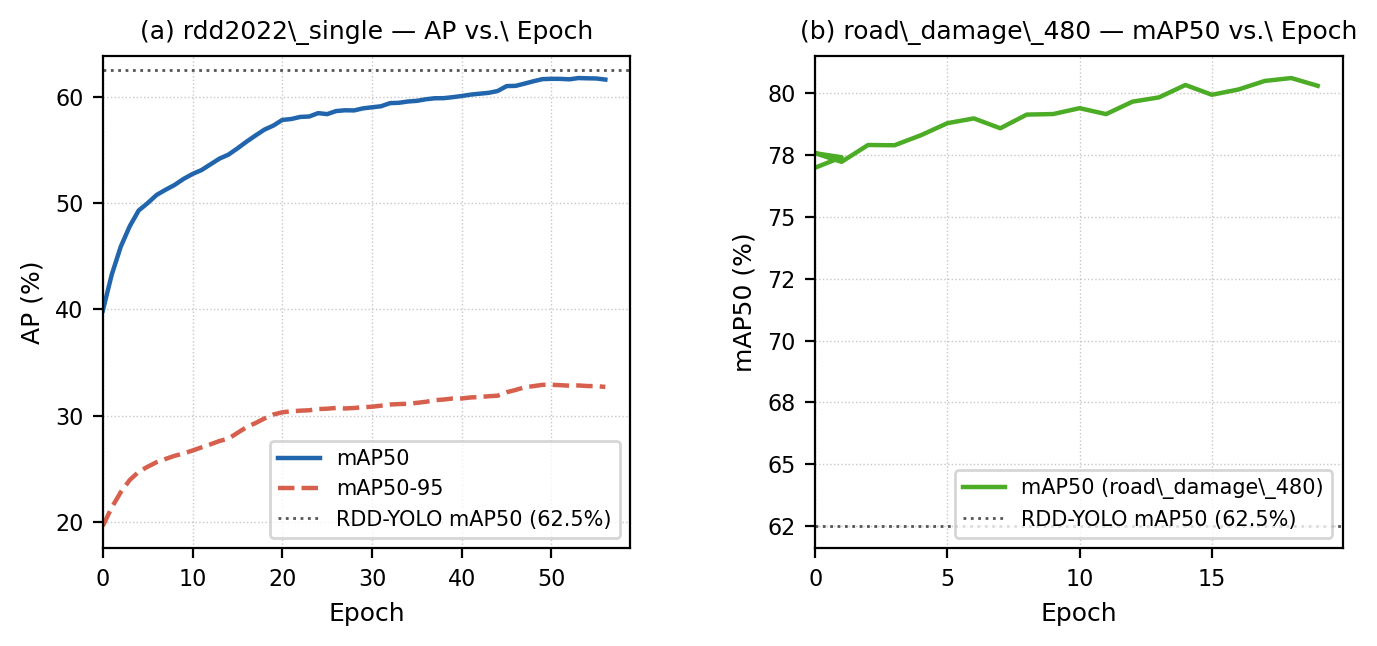
\includegraphics[width=\columnwidth]{figures/fig5_training_curves.pdf}
  \caption{Training convergence curves.
           \textit{Left:} mAP50 and mAP50-95 vs.\ epoch for the rdd2022\_single
           model (full RDD2022 dataset, 55 epochs). The dashed grey line marks
           RDD-YOLO's mAP50 of 62.5\%.
           \textit{Right:} mAP50 convergence for road\_damage\_480 (curated
           subset, 20 epochs), surpassing RDD-YOLO from epoch 14 onward.}
  \label{fig:curves}
\end{figure}

The rdd2022\_single model reaches near-RDD-YOLO mAP50 within 55 epochs, compared
to the 180 epochs required by RDD-YOLO~\cite{rddyolo}, reflecting the efficiency
of transformer-based fine-tuning from strong COCO pretrained weights.
The road\_damage\_480 model surpasses the RDD-YOLO mAP50 baseline from epoch 14
onward on the curated validation set.

% -------------------------------------------------------
%  6. Discussion
% -------------------------------------------------------
\section{Discussion}
\label{sec:discussion}

\subsection{Efficiency--Accuracy Trade-off}

Our rdd2022\_single model achieves near-equivalent mAP50 (61.6\% vs.\ 62.5\%) at
70\% fewer parameters and 77\% fewer GFLOPs, with 3.6$\times$ faster training
convergence (50 vs.\ 180 epochs).
This parameter efficiency arises from the PResNet18 backbone, which provides
sufficient feature extraction capacity for a binary damage/background classification
task without the depth of the YOLOv8x backbone in RDD-YOLO.
The end-to-end transformer decoder further eliminates the NMS post-processing step
present in YOLO-series detectors, simplifying the inference pipeline.
The reduced compute budget suggests potential for deployment on hardware with
constrained resources such as vehicle-mounted inspection cameras or UAVs, though
runtime benchmarking on such platforms is left for future work.

\subsection{Single-Class vs.\ Multi-Class Formulation}

The single-class formulation trades per-category diagnostic granularity for
cross-category generalisation.
Our model detects all four damage morphologies without category-specific supervision,
which is advantageous in operational inspection settings where rapid flagging of any
damage type is the primary requirement.
A two-stage system---where the single-class detector provides a detection mask that is
then classified by a lightweight head---could recover per-category outputs without
sacrificing the recall advantages of the unified detector.
Such an architecture is left for future work.

\subsection{AR@50 as a Safety Metric}

AR@50\,=\,0.926 means the model recovers 92.6\% of all annotated damage instances at
IoU\,=\,0.50.
In road inspection contexts, undetected damage is a safety risk; a high-recall
detector that generates false positives for human review is preferable to a
high-precision detector that silently misses damage.
RDD-YOLO does not report AR, preventing direct comparison; we recommend that future
road damage detection papers include AR alongside mAP to enable safety-oriented
evaluation.

\subsection{Interpretability Analysis}

Eigen-CAM maps applied to the PResNet18 final convolutional layer show strong
activations along crack edges and pothole boundary regions, confirming that the
backbone has learned to represent structural damage geometry rather than background
road texture.
Deformable Attention sampling points from the transformer decoder are distributed
across both the damage boundary and interior, consistent with the model learning to
localise and delineate damage extents for accurate bounding box regression.
Together these visualisations provide evidence that the model's detections are grounded
in damage-relevant features, which is important for acceptance of automated inspection
systems in safety-critical applications.

\subsection{Limitations}

The following limitations should be acknowledged:
\begin{enumerate}
  \item The single-class formulation eliminates per-category diagnostic output useful
        for infrastructure management databases.
  \item Our models are evaluated at 480$\times$480 resolution; RDD-YOLO evaluates at
        640$\times$640, making a direct resolution-equivalent comparison impossible
        without additional experiments.
  \item XAI analysis is qualitative; quantitative attribution studies (e.g.\ LIME,
        SHAP) are left for future work.
  \item Class imbalance in RDD2022 (D40 potholes are underrepresented relative to
        crack categories) may affect per-category recall under any class-conditional
        evaluation.
  \item The rdd2022\_single model was still training at submission time (epoch 49 of
        75); final epoch results may show further improvement.
\end{enumerate}

% -------------------------------------------------------
%  7. Conclusion
% -------------------------------------------------------
\section{Conclusion}
\label{sec:conclusion}

We have presented an efficient road damage detection system built on the RT-DETRv2
transformer architecture fine-tuned on the RDD2022 benchmark.
Using a PResNet18 backbone with approximately 20\,M parameters and 60\,GFLOPs, our
model achieves mAP50\,=\,61.6\% and AR@50\,=\,0.926 on the full RDD2022 validation
set under a single-class formulation, with 70\% fewer parameters and 77\% fewer
GFLOPs than the CNN-based RDD-YOLO baseline.
A curated-subset variant achieves mAP50\,=\,80.3\%.
Eigen-CAM and Deformable Attention visualisations confirm that the model learns
damage-relevant structural features rather than road texture, supporting its
applicability in safety-critical inspection workflows.

Future directions include:
(i) a two-stage system adding a per-category classification head on top of the
single-class detector;
(ii) quantitative attribution analysis using LIME or SHAP;
(iii) evaluation of larger backbone variants (PResNet34, PResNet50) to establish an
accuracy ceiling for transformer-based road damage detection;
and (iv) runtime evaluation at higher input resolutions for cross-resolution
comparison with CNN baselines.

% -------------------------------------------------------
%  References
% -------------------------------------------------------
\bibliographystyle{IEEEtran}
\bibliography{references}

\end{document}
